\setchapterstyle{kao}
\setchapterpreamble[u]{\margintoc}

\chapter{Standard Model Background Simulation and Data Processing}
\labch{simulation_and_processing}



\section{Event Generation}

\subsection{Neutrinos}

\subsection{Muons}



\section{Detector Simulation}

\subsection{Photon Propagation}

\subsection{Detector Respones}


\section{Processing}

\subsection{Trigger and Online Filter}

\subsection{Offline Filter}


\subsection{Hit Selection} \labsec{hit_selection}

To select hits that originated from direct photons, a procedure closely related to the one described in \sidecite{JPGarza} is applied.
The cleaning is based on removing hits from DOMs that could have originated from light emitted by any of the other hit DOMs on the same string.
The selection solely uses the time of arrival (TOA) of the pulses. It is carried out for every detected event in the following steps:

\begin{enumerate}[label=(\roman*)]
    \item Select strings where at least 3 DOMs have seen light.
    \item Every hit DOM is characterized by the time of the earliest pulse (above a threshold of 0.1\,photoelectron (PE)) and the integrated charge of all pulses.
    \item For every string passing these criteria the following steps are performed:
    \begin{enumerate}[label=(\alph*)]
        \item Remove DOMs with hit outside of a time window of [-250\,ns, +2000\,ns] around the median TOA of all hits on the string.
        \item Using the DOM with the highest charge as reference (estimate for point of closest approach), check if any of the other DOMs on the string lies in the time window
        \begin{equation}
            \left [ t_r - \frac{d_{r,i}}{c_\mathrm{ice}} - t_\mathrm{delay}, t_r + \frac{d_{r,i}}{c_\mathrm{ice}} + t_\mathrm{delay} \right ],
        \end{equation}
        where $t_r$ is the TOA of the reference DOM, $d_{r,i}$ is the absolute distance between the two DOMs considered, $c_\mathrm{ice}$ is the speed of light in ice and $t_\mathrm{delay}$ is the allowed time delay.
        A time delay of 20\,ns is used to limit the selection to photons with little scattering.
        \item For each of the selected DOMs, it is now verified that, compared to each of the other selected DOMs, none was hit after the time $t_\mathrm{max}$
        \begin{equation}
            t_\mathrm{max} = t_i + \frac{d_{i,j}}{c_\mathrm{ice}} + t_\mathrm{delay},
        \end{equation}
        where the subscripts $i$ and $j$ stand for the two DOMs in questions, and all combinations are checked.
        \item As the last step, it is checked whether there are more than six empty modules between selected modules.
        Keeping the DOM with the largest charge, the other DOMs are checked going upwards and downwards along the string.
        Finally, only strings that still have three or more selected DOMs are kept and their hits are identified as direct pulses.
    \end{enumerate}
\end{enumerate}


\subsection{Reconstruction} \labsec{reconstruction}

There are several methods to select and reconstruct events in IceCube.
At energies around 10-40\,GeV, where we expect the oscillation signal, the events are faint and only a few DOMs detect light.
One approach for the reconstruction of such events is described in this section.
The reconstruction uses only photons that traveled along a straight line - called \textit{direct} photons.
Using direct photons has the benefit of reducing the systematic biases caused by the large variations of the bulk ice properties; scattering and absorption.
With an average distance of 70\,m between strings in DeepCore and an effective scattering length of about 50\,m \sidecite{LUNDBERG2007619}, there will always be a fraction of direct photons arriving at the DOMs.
The used method applies a stepwise procedure, where first a cleaning routine selects events with direct photons as described in Section \refsec{hit_selection}. 
Afterward, the direction of the particle is reconstructed and finally the energy is determined as outlined in Sections \refsec{flercnn_reconstruction}.


\subsubsection{FLERCNN Event Reconstruction and Classification} \labsec{flercnn_reconstruction}

Didn't copy over SANTA/LEERA since I need the FLERCNN desciption here.


\subsubsection{Standard Model Event Topologies}

The signals that IceCube detects vary depending on the neutrino flavor and interaction type of the event.
The two main signatures that can be observed are track-like and cascade-like events.
The observed Cherenkov light is produced by the secondary particles originating from the neutrino interactions described in Section \refsec{neutrino_interactions}.
Table \reftab{interactions_vs_signatures} shows an overview of the possible event signatures.
Minimum ionizing muons can travel for long distances and are seen as extended light signatures called tracks.
Muons can come from $\nu_\mu$-CC interactions or from $\nu_\tau$-CC followed by the decay of the $\tau$ to a muon.
However, the $\tau$ only decays to a muon with a branching ratio of BR=17\,\%.

Cascades are the light signal produced by the EM/hadronic showers described in Section \refsec{energy_loss}.
They come from $\nu_e$-CC and most of the $\nu_\tau$-CC interactions because the electron and the tau lose all their energy quickly and only travel a short distance.
They are also produced in all $\nu$-NC interactions since only the hadronic shower is observable and the produced neutrino escapes unseen.
The cascades at the energies considered in this work have a smaller radius than the spacing of the DOMs and are therefore seen as point-like light emitters.

% \begin{table}[h]
%     \small
%     \begin{center}
%         \begin{tabular}{  m{2.3cm} m{2.3cm} m{4.5cm} m{3.5cm}  } 
%             \hline\hline
%             \textbf{Interaction} & \multicolumn{2}{c}{\textbf{Secondary particles}} &\textbf{Signature} \\ 
%             \hline\hline
%             \multirow{2}{*}[-1.5em]{CC $\overset{\scriptscriptstyle(-)}{\nu_\mu}$ }
%             & 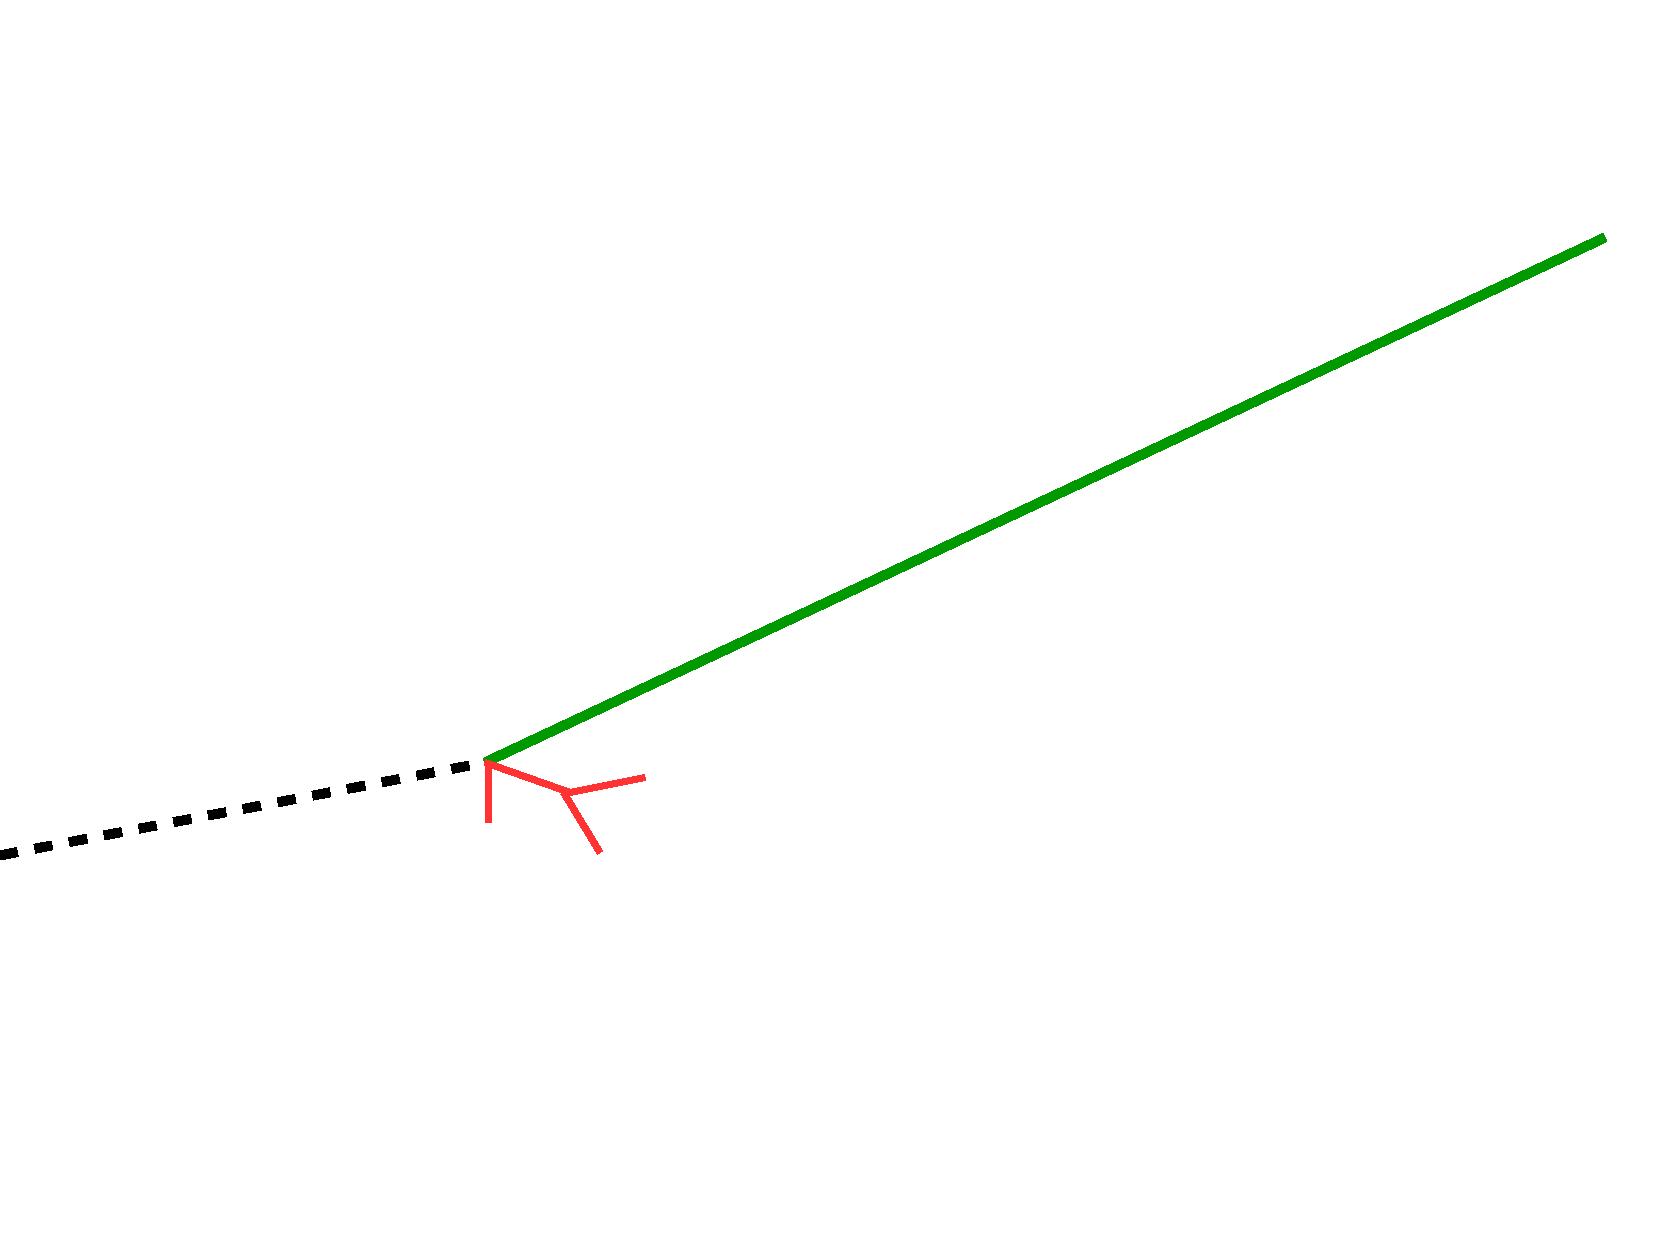
\includegraphics[width=2cm]{figures/neutrinos_properties/interaction_schematics/numu_CC_muon_only.pdf} 
%             & $\mu^\pm$ track 
%             & Track-only  \\
%             \cmidrule{2-4} 
%             &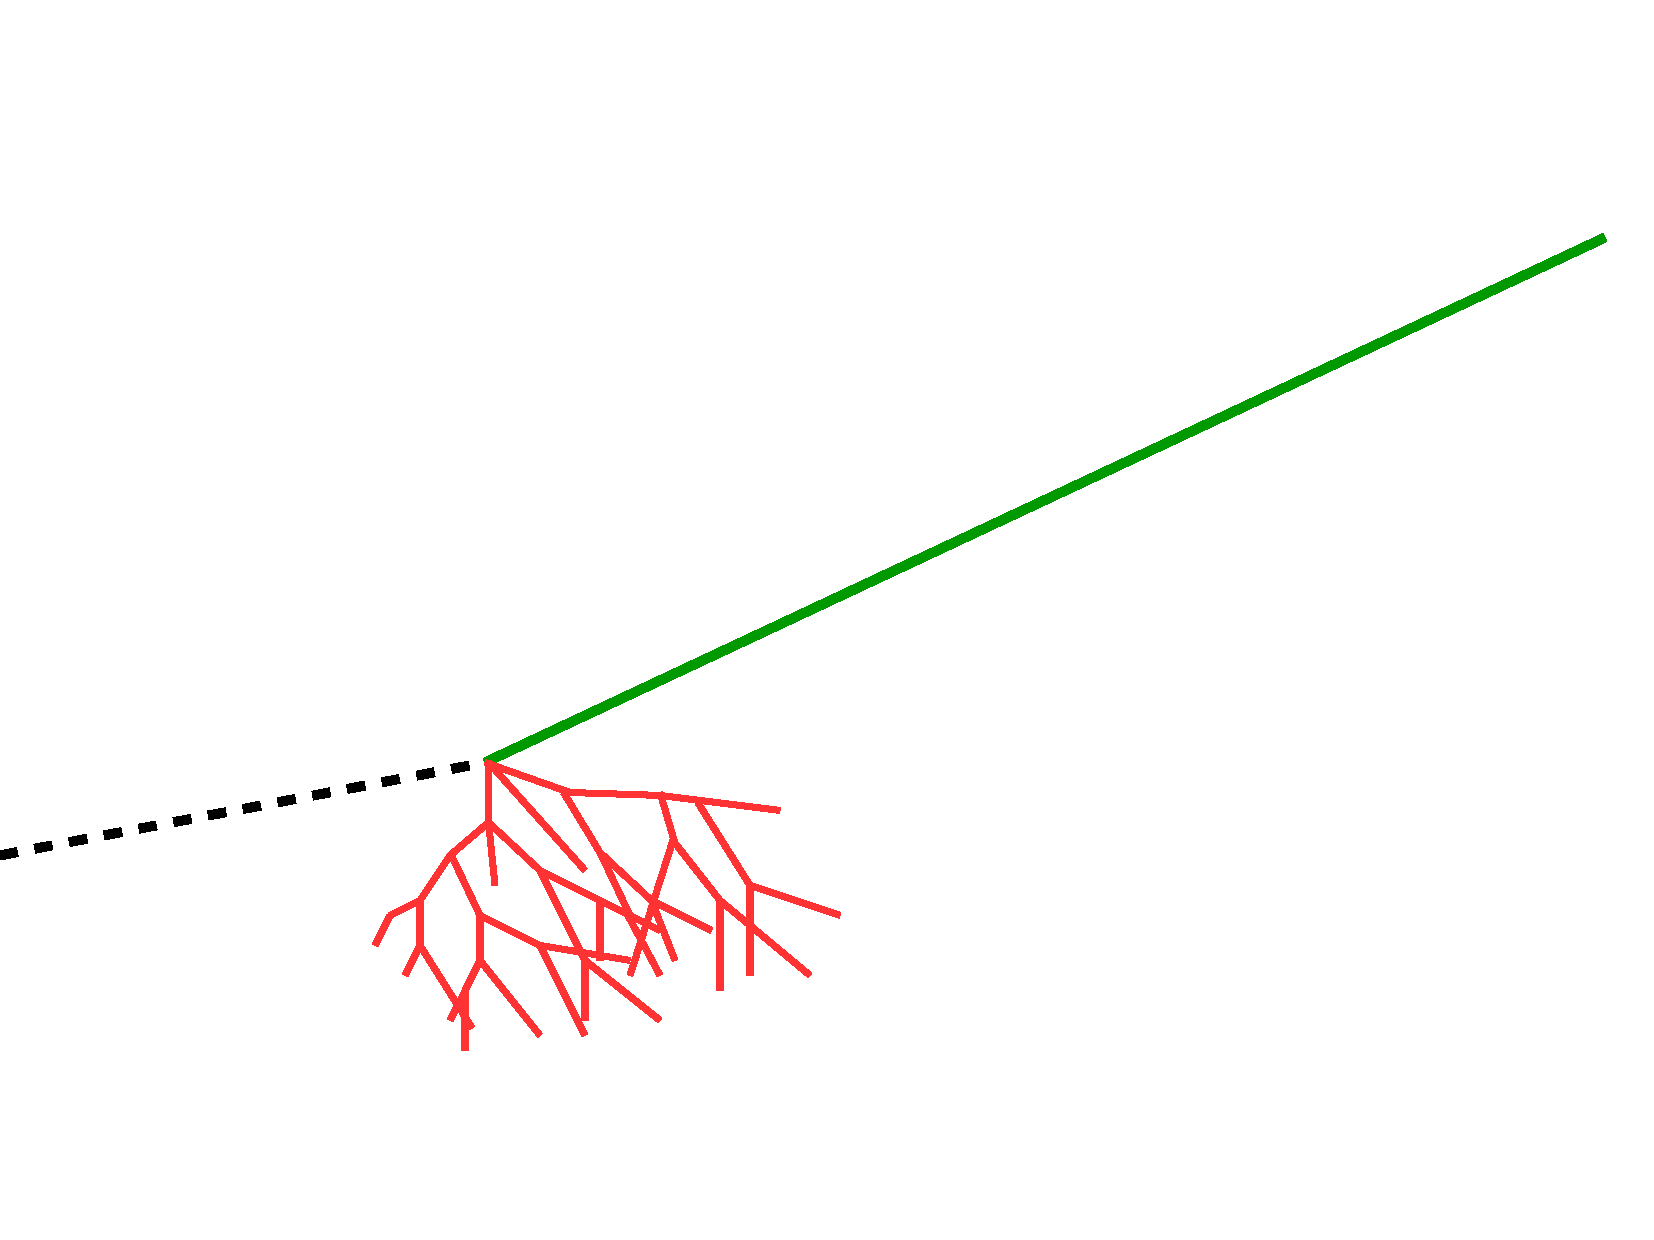
\includegraphics[width=2cm]{figures/neutrinos_properties/interaction_schematics/numu_CC_track_cascade.pdf}  
%             & $\mu^\pm$ track and hadrons 
%             & \multirow{2}{*}[-2em]{Track with cascade} \\
%             \cmidrule{1-3}
%             \multirow{2}{*}[-1.5em]{CC $\overset{\scriptscriptstyle(-)}{\nu_\tau}$ }
%             &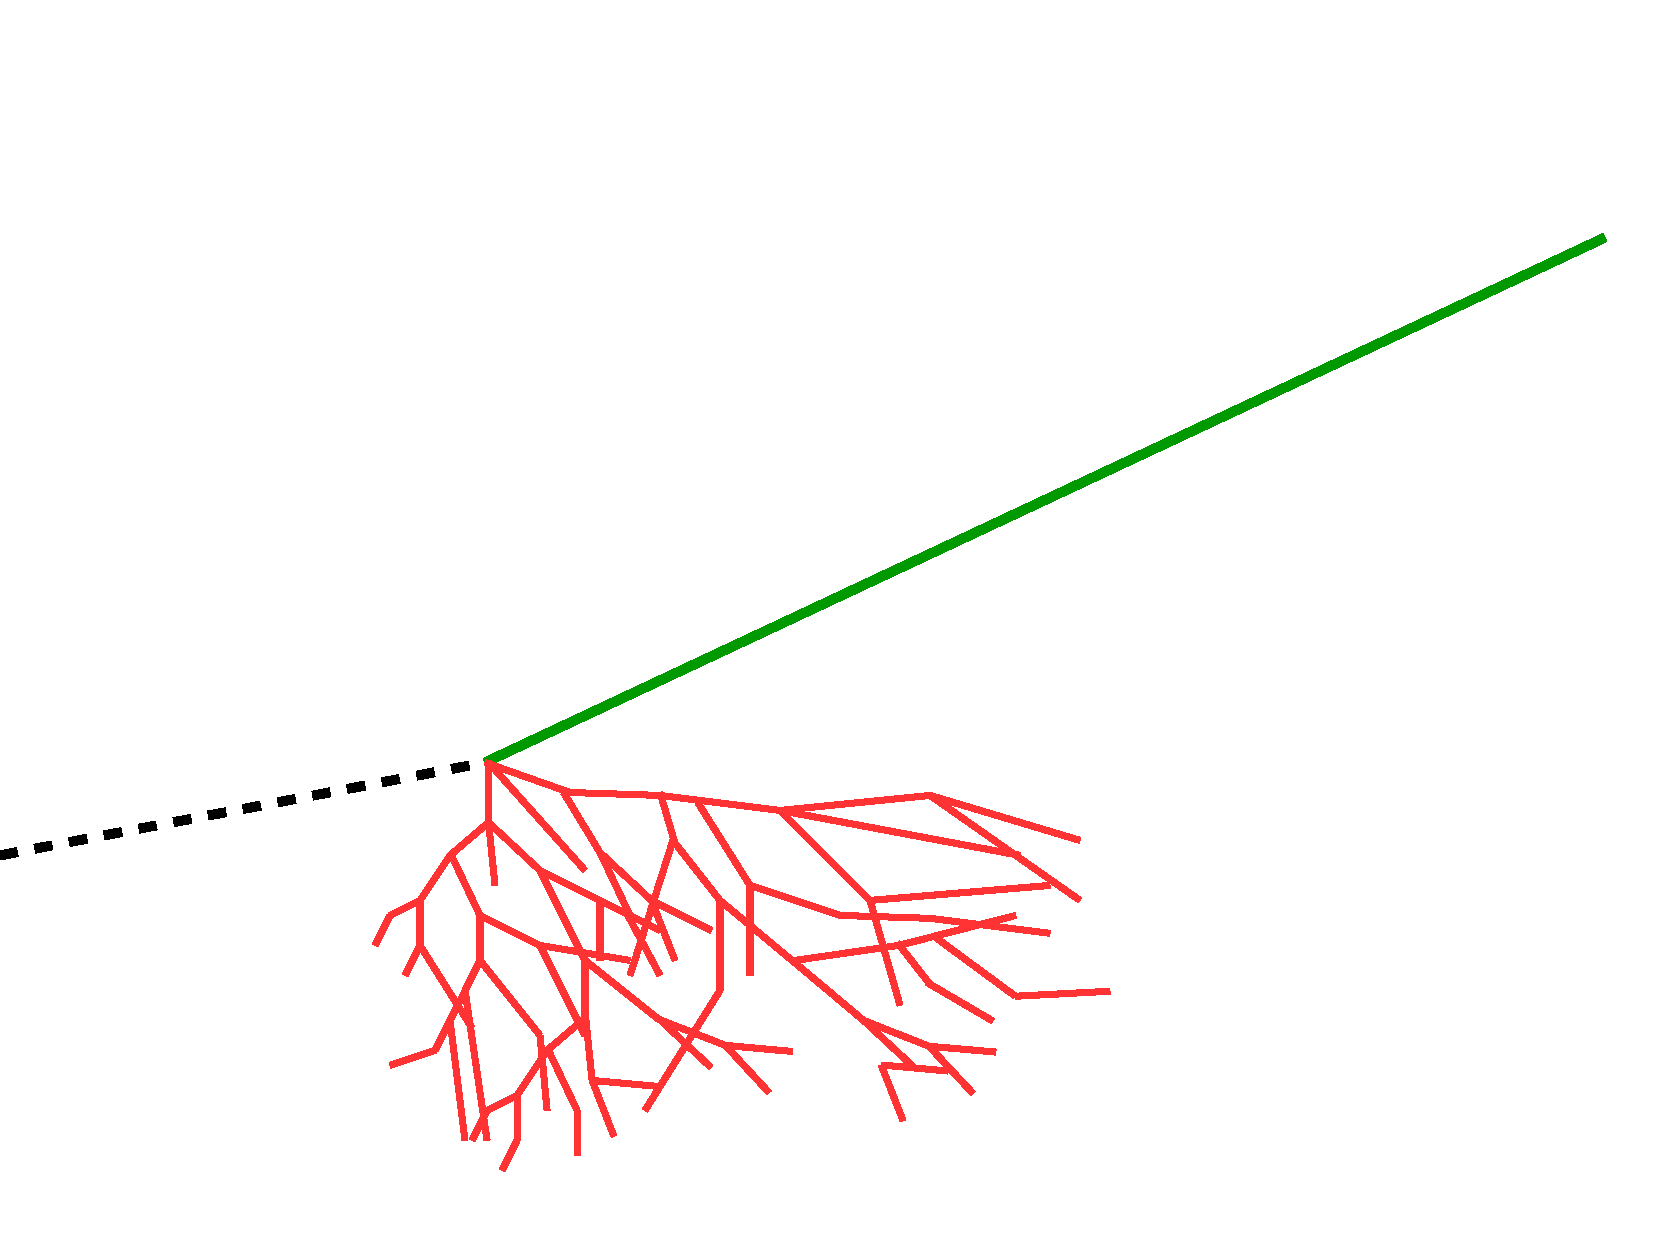
\includegraphics[width=2cm]{figures/neutrinos_properties/interaction_schematics/nutau_CC_track_cascade.pdf} 
%             & $\tau^\pm$ decaying into $\mu^\pm$ ($\sim$17\% BR), hadrons 
%             & {}\\
%             \cmidrule{2-4}
%             & 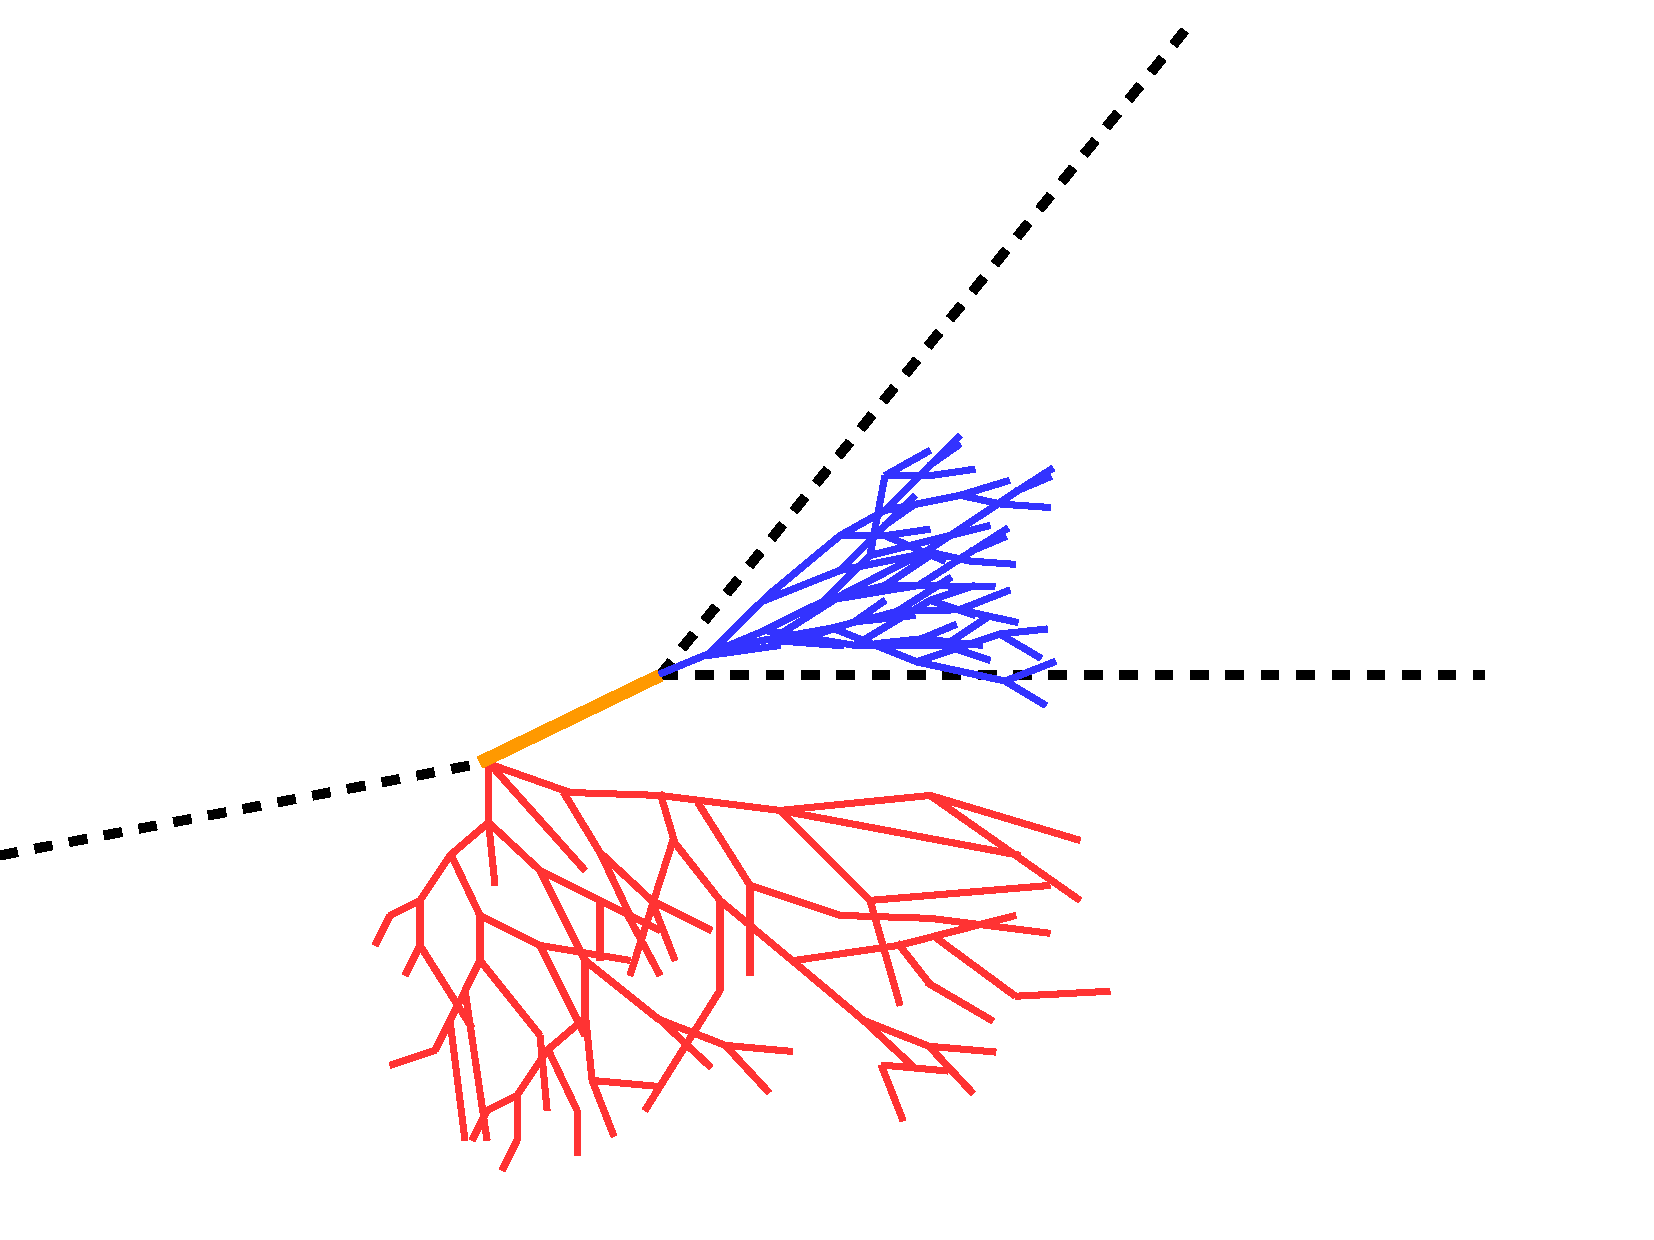
\includegraphics[width=2cm]{figures/neutrinos_properties/interaction_schematics/nutau_CC_cascadeonly.pdf}
%             & $\tau^\pm$ decaying into $e^\pm$ or hadrons ($\sim$83\% BR)  
%             & {}\\
%             \cmidrule{1-3} CC $\overset{\scriptscriptstyle(-)}{\nu_e}$ 
%             & 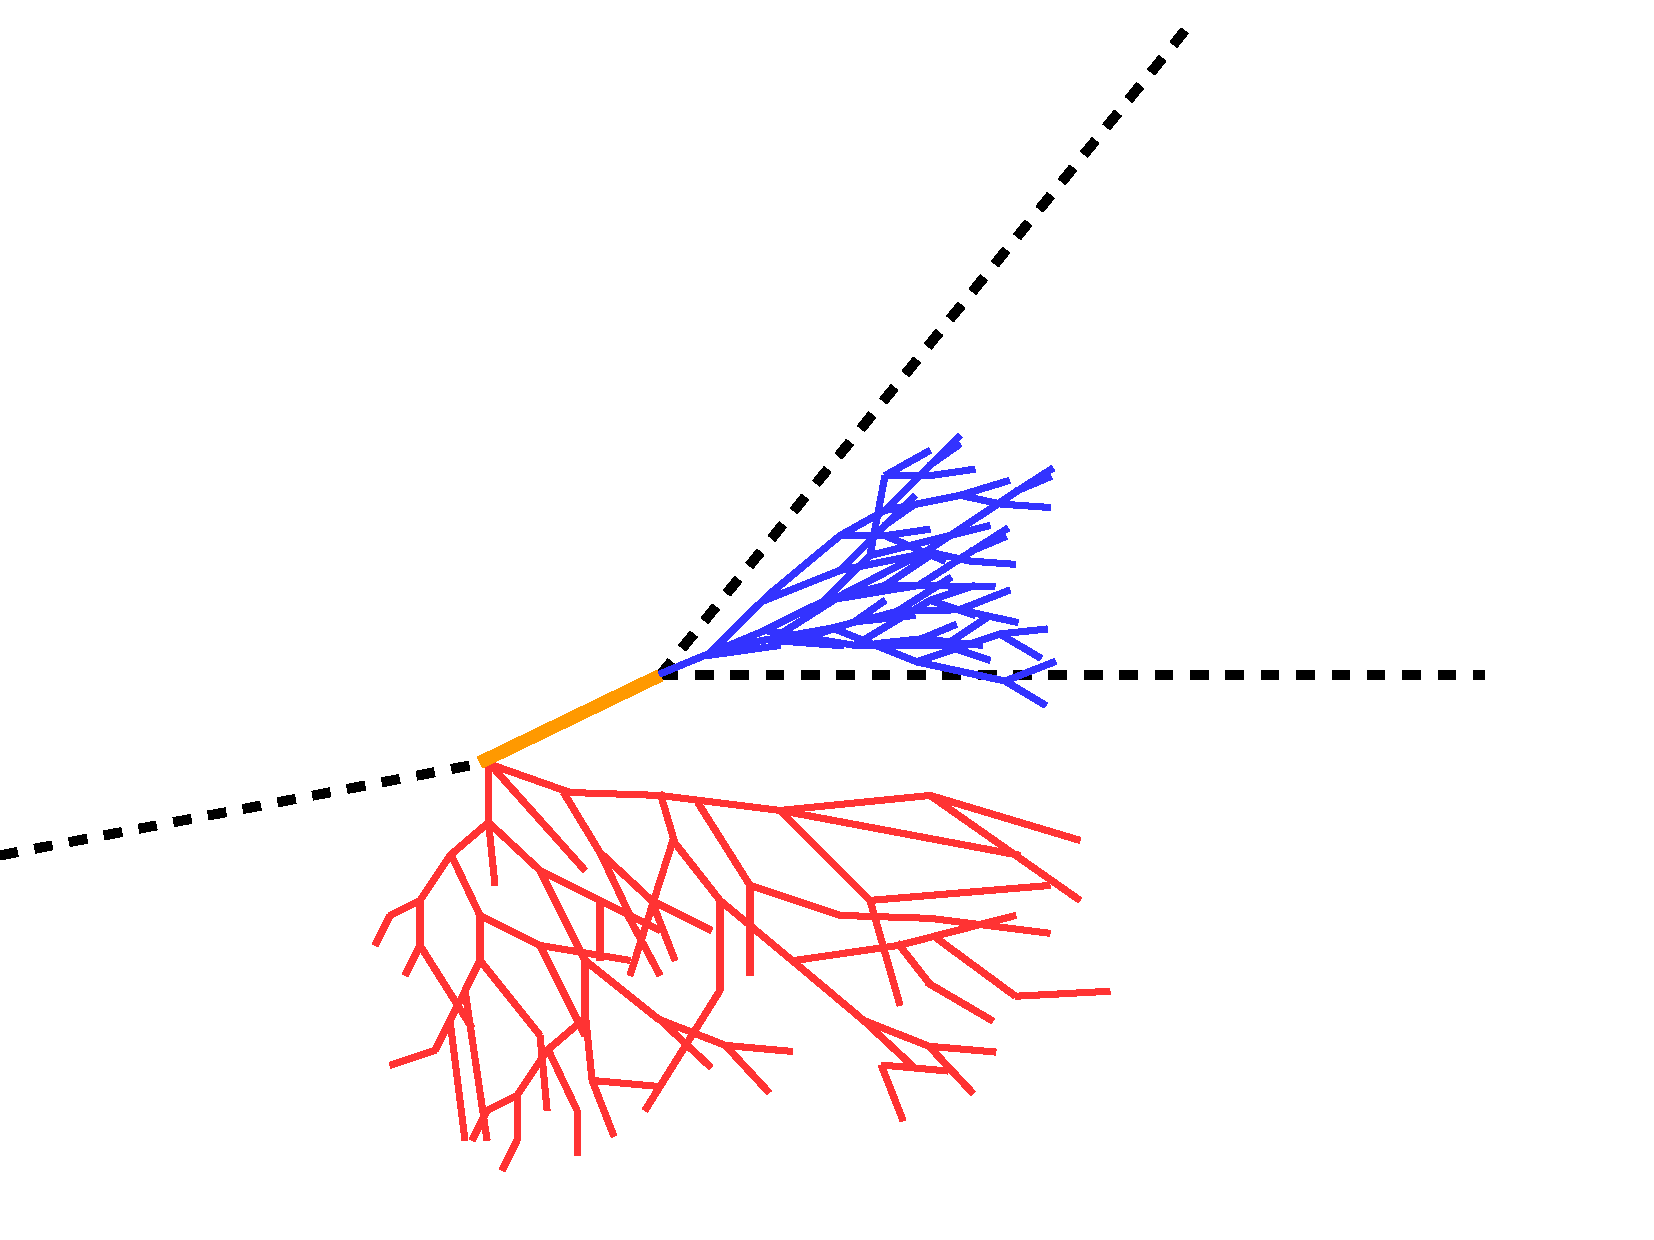
\includegraphics[width=2cm]{figures/neutrinos_properties/interaction_schematics/nue_CC_cascadeonly.pdf}
%             & $e^\pm$, hadrons & {Cascade-only}\\
%             \cmidrule{1-3}
%             NC $\overset{\scriptscriptstyle(-)}{\nu_\ell}$ 
%             & 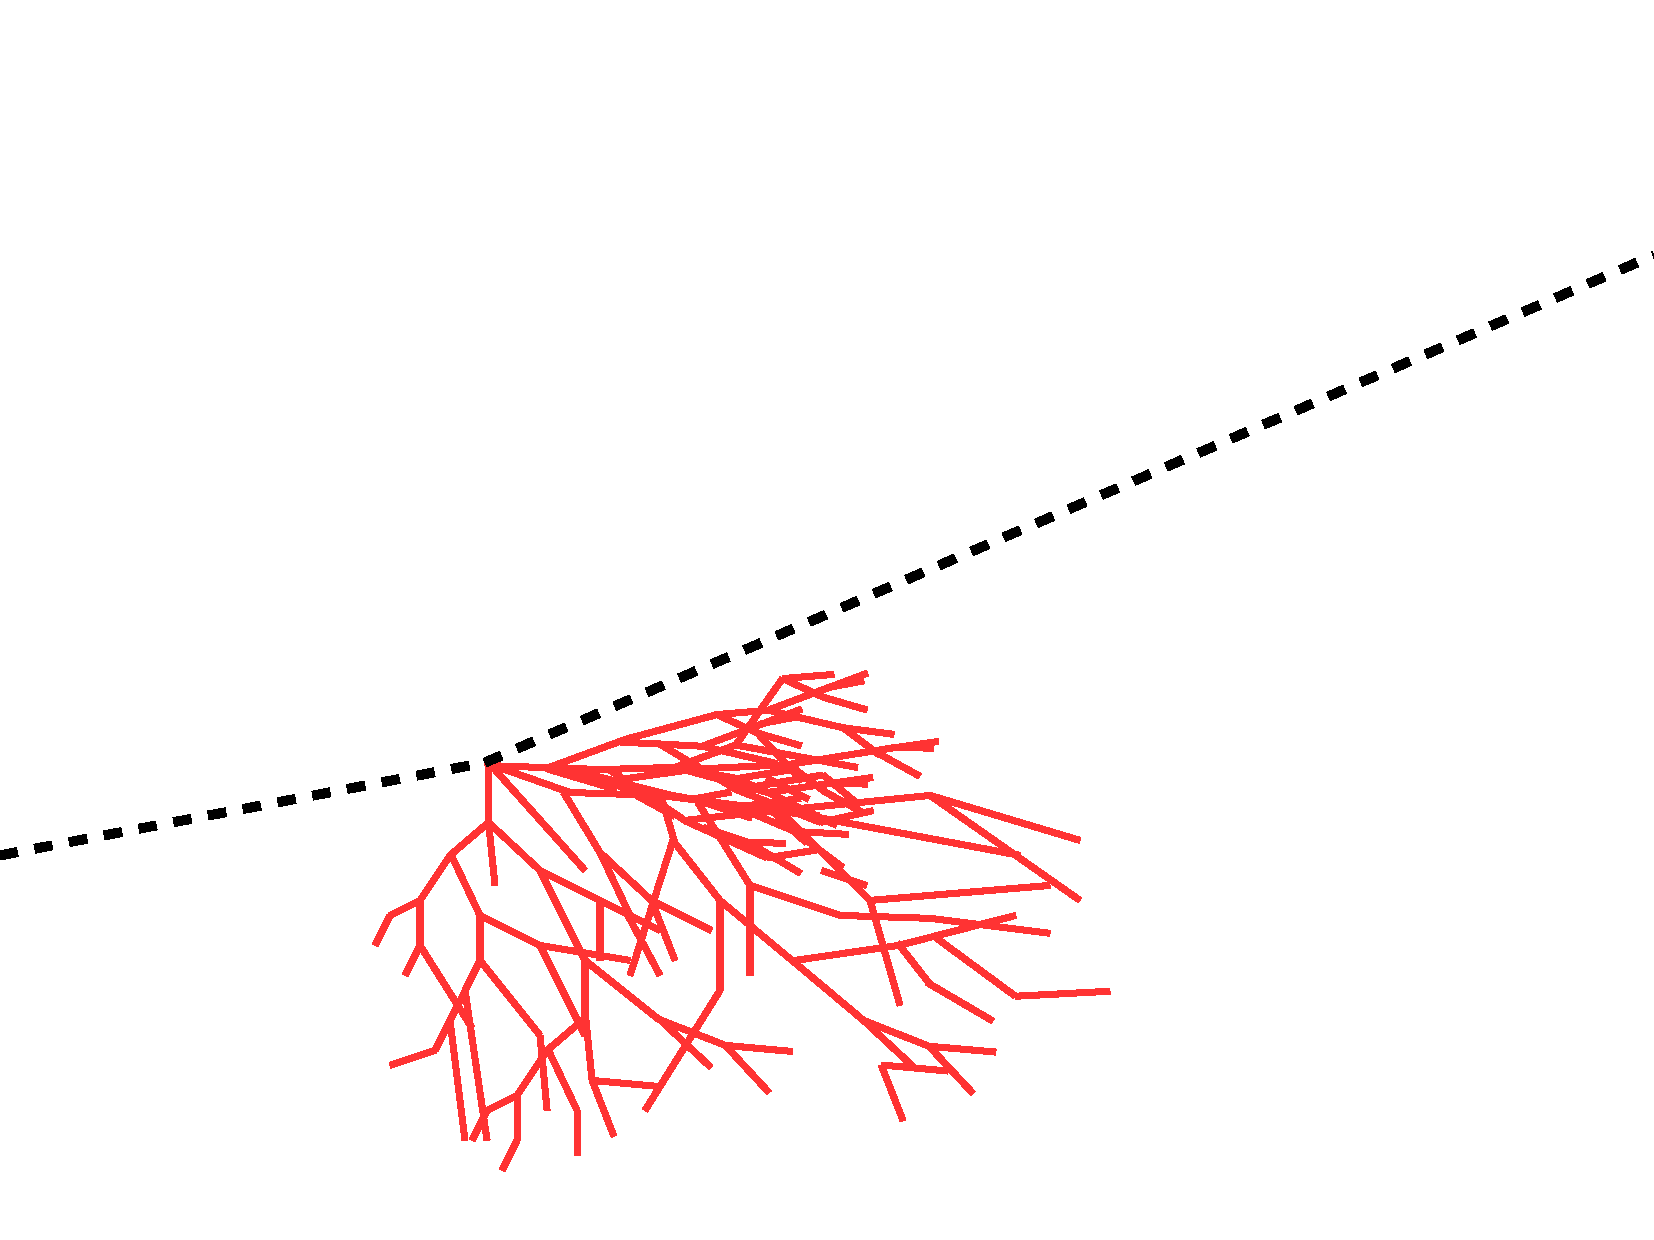
\includegraphics[width=2cm]{figures/neutrinos_properties/interaction_schematics/nuall_NC_cascadeonly.pdf} 
%             & hadrons &  {} \\
%             \hline
%         \end{tabular}
%     \end{center}
%     \caption[Event signatures in IceCube and their underlying interactions, taken from~\sidecite{ATerliuk}]{IceCube event signatures, their underlying interaction type and the particles that produce them. Also shown are the secondary particles produced in the interactions. Black dashed lines represent neutrinos, green lines muons, and blue and red lines are particles in electromagnetic and hadronic cascades, respectively. Taken from~\sidecite{ATerliuk}.}
%     \labtab{interactions_vs_signatures}
% \end{table}

The existence of the two types of event topologies and their origins imply that by identifying track-like events we can identify events coming (mainly) from $\nu_\mu$-CC interactions and therefore obtain a flavor identification.
This is a crucial part of performing an oscillation analysis as will be further discussed in Section \refsec{analysis_principle}.



\section{Systematic Uncertainties}

\subsection{Detector Property Variations}

\subsection{Atmospheric Flux}
